\section{Comparing expansions, factor reductions, and quantisers}\label{sec:methods_vtwo}
A deterministic \RoughCert{} enclosure supports two decisions. For a method value enclosed in $[A,B]$ and a
continuous-model bracket $[L,U]$, the signed pricing error lies in $[A-U,B-L]$. The method is certified
tick-accurate when that interval fits inside $[-0.05,0.05]$, and certified biased when it lies strictly on
one side of zero, which is the disjointness used throughout this section; calls use the same $0.05$-point
price tolerance, and implied-volatility differences are measured in percentage points.

\subsection{The exercise boundary and direct implied volatility}\label{sec:direct_expansion}
In the mixed expansion of \citet[Theorem~3.1]{BourgeyDeMarcoGobet2023}, let
$y_j(z)=\bar\xi\,\lambda_j\exp(\mu_j+s_jz)$ and $Y(z)=y_1(z)+y_2(z)$, where
$\bar\xi=\Delta^{-1}\int_T^{T+\Delta}\xi_0(u)\dd u$. For a fixed strike $K>0$, $Y(z)=K^2$ has a unique root
for positive amplitudes. The weak derivative of the call under a shift in component $j$ is
$y_j(z)\mathbf{1}_{\{Y(z)>K^2\}}/(2\sqrt{Y(z)})$. Integrating against the normal density times
$\gamma_{1,j}+\gamma_{2,j}z/s_j+\gamma_{3,j}(z^2-1)/s_j^2$ and adding the proxy call evaluates the
published coefficient expression rigorously (the exercise boundary has zero normal mass; the original mixed
theorem states its remainder for smooth payoffs).

At $k=-0.20$, the authors' implementation---$100$-node Gauss--Hermite quadrature with $10^{-4}$
finite-difference derivatives---yields $93.326\%$, whereas splitting
the integral at exercise in Arb gives $[93.8671,93.8672]\%$ against a \RoughCertCV{} band of
$[93.9407,94.2487]\%$. At $k=+0.10$ the corresponding values are $96.768\%$, $[97.0817,97.0818]\%$, and
$[97.1870,97.3764]\%$. All seven root-split IVs fall strictly below the lower edge, with edge separations of $\MixSplitSepLo$ to
$\MixSplitSepHi$ percentage points, while that $100$-node implementation adds a separate strike-dependent
kink oscillation (Figure~\ref{fig:methoderrors}(a)).

For a single kernel, equation~(21) of \citet{LiaoAgarwalBourgey2026} gives the direct IV formula
\[
 \widehat\sigma(K)=\frac{v}{2}+\frac{\gamma_2}{2vT}+\frac{3\gamma_3}{8vT}
                 -\frac{\gamma_3\log(S/K)}{v^3T^2},
 \qquad v=\frac{\norm{h_0^{(a)}}}{\sqrt{T}},
\]
where $S$ is the zeroth-order VIX forward and $h_0^{(a)}$ is the barycentre with amplitude $a$. Fixing
physical strikes via the order-three forward on the authors' $\Delta=30/365$ window and enclosing both
the direct formula and the continuous model in 169-bit Arb establishes a downward IV bias at all $30$
strikes for $H=0.10$, at $22$ of $30$ strikes for $H=0.23$, and at all $6$ stress strikes
(Table~\ref{tab:competitors}, Panel~A; the remaining eight comparisons overlap, with zero strikes above).

\begin{figure}[!htbp]\centering
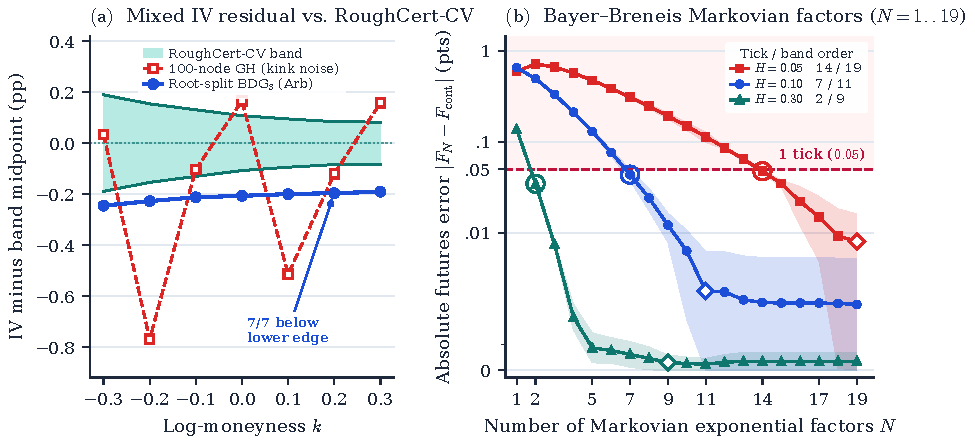
\includegraphics[width=\textwidth]{figures/fig_v3_05_mixed_and_markov.pdf}
\caption{(a) Mixed-smile IV deviations from the continuum midpoint. (b) Absolute futures-error enclosures and midpoints for $N=1,\ldots,19$. Circles mark one-tick accuracy and diamonds mark containment in the fixed continuum band.}\label{fig:methoderrors}
\end{figure}

\subsection{Markovian factor count and product quantisation}\label{sec:factor_counts}
We evaluate the geometric Gaussian rule and numerical $L^2$ kernel optimisation of
\citet{BayerBreneis2023}, freezing the returned positive nodes and weights at their recorded decimal values.
For $K_N(t)=\sum_j w_j e^{-\gamma_j t}$, the finite model has exact covariance
\[
 C_N(x,y)=\sum_{i,j} w_i w_j e^{-\gamma_i x-\gamma_j y}\,\frac{1-e^{-(\gamma_i+\gamma_j)T}}{\gamma_i+\gamma_j},
\]
with the quotient read as $T$ when $\gamma_i+\gamma_j=0$, enabling verified \RoughCertCV{} enclosures of every $N$-factor model. On the flat
three-month contract ($a=1$, $\Delta=1/12$, $\xi_0=0.235^2$), the Arb-proved minimum optimised factor counts
achieving $<0.05$-point futures error are $14$, $7$, and $2$ for $H=0.05$, $0.10$, and $0.30$
(Figure~\ref{fig:methoderrors}(b); Table~\ref{tab:competitors}, Panel~B), with every smaller integer proved
outside. For full containment inside the fixed continuum band ($M=144$, $N_z=320$), the proved minimum
orders are $19$, $11$, and $9$ (with every smaller integer proved disjoint from that fixed band). At $H=0.05$, conditioning the
tilted residual on the contrast $k_{\Delta/14}-k_\Delta$ cleanly separates the $13$-factor error
$[-0.0671,-0.0611]$ from the $14$-factor error $[-0.0496,-0.0453]$. On the three fixed-strike calls
($K\in\{18,22,26\}$), all minimum orders are exact at $H=0.10$ and $0.30$, while at $H=0.05$ two strikes
leave a one-factor overlap bracket ($N\in\{5,6\}$ at $K=18$ and $N\in\{1,2\}$ at $K=22$, noted explicitly in
Table~\ref{tab:competitors}). These thresholds apply to the recorded fitting horizon $T+\Delta$, nodes, and
weights rather than all possible positive exponential sums.

The functional quantiser of \citet[Remark~4.9]{BonesiniCallegaroJacquier2023} expands the Brownian input in
cosines on $[0,T+\Delta]$ while retaining continuous Gaussian variance compensation. Using their Table~1
allocations at budgets $100$ and $1000$ (and declared allocations $(6,4,2)$ and $(10,4,3,2,2)$ at $50$ and
$500$), we enclose both scalar normal centroids and delivery integrals in Arb. Even at $960$ product paths,
all $18$ literature futures prices are underestimated by at least $0.208$ points on $\Delta=1/12$ (and by
$0.209$--$1.412$ points on $\Delta=30/365$; Table~\ref{tab:competitors}, Panel~C; Figure~\ref{fig:scoreboard}(b)).
A separate forward-field Karhunen--Lo\`eve diagnostic in the archive assesses basis choice across two
delivery grids.

\begin{table}[!htbp]\centering\scriptsize\setlength{\tabcolsep}{3.3pt}
\caption{Multi-method competitor audit against \RoughCertCV{} across direct IV expansions (LAB~2026), Markovian factor reductions (Bayer--Breneis), and product functional quantisation (BCJ~2023).}\label{tab:competitors}
\begin{tabular}{@{}lcccccc@{}}\toprule
\multicolumn{7}{@{}l}{\emph{Panel A: Direct implied-volatility expansion \citep[Eq.~(21)]{LiaoAgarwalBourgey2026} against \textbf{\RoughCertCV{}}}} \\
\addlinespace[1.5pt]
 & & & \multicolumn{3}{c}{Comparison with \textbf{\RoughCertCV{}}} & \\
\cmidrule(lr){4-6}
Regime & $H$ & Maturity & Strikes below & \shortstack{Strikes\\overlapping} & \shortstack{Max shortfall\\(pp)} & Verdict \\\midrule
LAB author grid & 0.10 & 1\,m & 10/10 & 0/10 & 0.487 & All below \\
LAB author grid & 0.10 & 3\,m & 10/10 & 0/10 & 0.236 & All below \\
LAB author grid & 0.10 & 6\,m & 10/10 & 0/10 & 0.140 & All below \\
LAB author grid & 0.23 & 1\,m & 10/10 & 0/10 & 0.021 & All below \\
LAB author grid & 0.23 & 3\,m & 8/10 & 2/10 & 0.008 & 2 overlap \\
LAB author grid & 0.23 & 6\,m & 4/10 & 6/10 & 0.002 & 6 overlap \\
Stress ($\eta_{\mathrm{P1}}=3$) & 0.10 & 6\,m & 6/6 & 0/6 & 0.435 & All below \\
\midrule
\multicolumn{7}{@{}l}{\emph{Panel B: Bayer--Breneis Markovian factor thresholds ($T=3$\,m, $a=1.0$, $\Delta=1/12$, $\xi_0=0.235^2$)}} \\
\addlinespace[1.5pt]
Hurst $H$ & \shortstack{Futures\\within tick} & \shortstack{Futures inside\\reference band} & Call $K=18$ & Call $K=22$ & Call $K=26$ & Verification \\\midrule
0.05 & 14 & 19 & 5 or 6$^\dagger$ & 1 or 2$^\dagger$ & 1 & Exact except $^\dagger$ \\
0.10 & 7 & 11 & 2 & 1 & 5 & All exact minima \\
0.30 & 2 & 9 & 1 & 2 & 2 & All exact minima \\
\midrule
\multicolumn{7}{@{}l}{\emph{Panel C: BCJ~(2023) product functional quantisation signed futures errors (pts) and median runtimes (s)}} \\
\addlinespace[1.5pt]
Budget / Paths & \multicolumn{2}{c}{18-cell ($\Delta=1/12$)} & 18-cell ($30/365$) & Stress (pts) & Setup (s) & Price (s) \\\midrule
50 / 48 & \multicolumn{2}{c}{[$-$2.077,\,$-$0.321]$^\star$} & [$-$2.092,\,$-$0.322]$^\star$ & [$-$1.239,\,$-$1.219]$^\star$ & 0.12 & 0.07 \\
100 / 96 & \multicolumn{2}{c}{[$-$1.851,\,$-$0.280]$^\star$} & [$-$1.863,\,$-$0.282]$^\star$ & [$-$1.184,\,$-$1.164]$^\star$ & 0.12 & 0.14 \\
500 / 480 & \multicolumn{2}{c}{[$-$1.450,\,$-$0.216]$^\star$} & [$-$1.458,\,$-$0.216]$^\star$ & [$-$0.994,\,$-$0.972]$^\star$ & 0.14 & 0.71 \\
1000 / 960 & \multicolumn{2}{c}{[$-$1.406,\,$-$0.208]$^\star$} & [$-$1.412,\,$-$0.209]$^\star$ & [$-$0.965,\,$-$0.942]$^\star$ & 0.17 & 1.42 \\
\bottomrule\end{tabular}
\smallskip\par\raggedright\scriptsize\emph{Notes:} Panel A counts implied-volatility intervals against the bold reference method; pp means percentage points. Panel B gives minimum factor counts. $^\dagger$ marks unresolved adjacent counts. Panel C gives quantiser minus continuum futures by window and budget. $^\star$ marks an entire error range beyond one Cboe tick ($0.05$ pts).
\end{table}
%

\subsection{Common curved contract scoreboard and numerical refinements}\label{sec:curved_score}
Table~\ref{tab:common} and Figure~\ref{fig:scoreboard}(a) compare all eight methods on a single curved
forward-variance contract ($H=0.10$, $T=3$\,m, $\Delta=1/12$, $a=1.9\sqrt{2H}$, $\xi_0(t)=0.234^2(1+t)^2$,
strike $K=27$). The $12$-factor futures, call and IV enclosures each overlap the continuum band.
The $500$-cell forward lies $0.00098$--$0.00999$ points above it. The lognormal future is more than one
tick low, while its IV is $1.26$--$1.76$ percentage points high. The $960$-path BCJ future is
$0.425$--$0.438$ points low and its IV is $5.51$--$5.86$ percentage points low. The BDG and LAB
curved-kernel IV enclosures both overlap the continuum interval. Their numerical point evaluations,
$96.821\%$ and $96.827\%$, lie approximately $0.14$ and $0.13$ percentage points below its lower edge;
the certified comparisons leave the sign unresolved.

\begin{figure}[!htbp]\centering
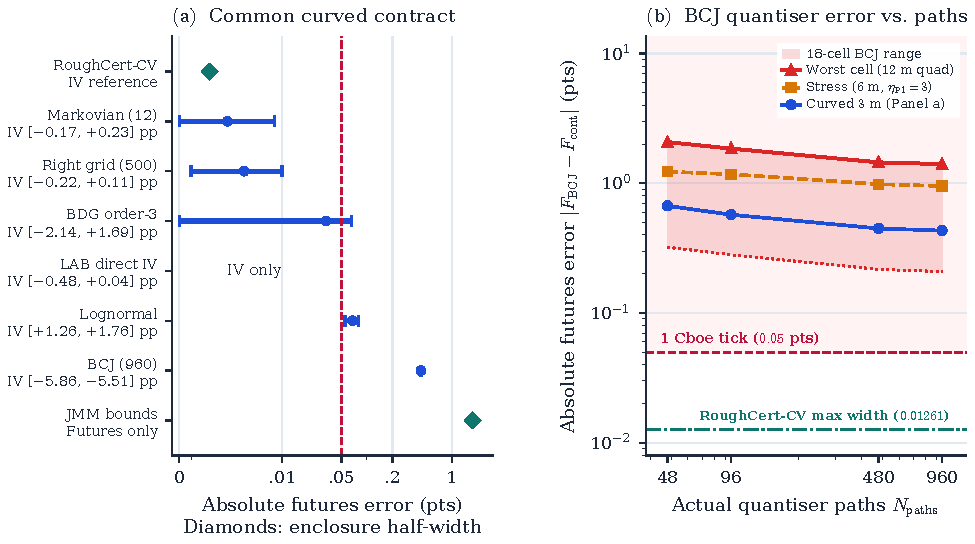
\includegraphics[width=\textwidth]{figures/fig_v3_06_scoreboard_and_quantizer.pdf}
\caption{(a) Curved contract at $K=27$. Bars enclose absolute futures errors, diamonds indicate enclosure half-widths, and row labels give signed IV differences from the continuum in percentage points. (b) BCJ quantisation error across four budgets and the largest 18-cell \RoughCertCV{} width.}\label{fig:scoreboard}
\end{figure}

\begin{table}[!htbp]\centering\scriptsize\setlength{\tabcolsep}{3.4pt}
\caption{Eight-method comparison on a common curved forward-variance contract ($H=0.10$, $T=3$\,m, $\Delta=1/12$, $\xi_0(t)=0.234^2(1+t)^2$, strike $K=27$ pts).}\label{tab:common}
\begin{tabular}{@{}lccccr@{}}\toprule
 & & \multicolumn{3}{c}{Outward-rounded enclosures at the same strike} & \\
\cmidrule(lr){3-5}
Method & Engine & Futures (pts) & Call (pts) & Black-76 IV (\%) & Against reference \\\midrule
\textbf{\RoughCertCV{} (continuum)} & Arb & \textbf{\boldmath [26.8389,\,26.8441]} & \textbf{\boldmath [5.078,\,5.085]} & \textbf{\boldmath [96.95,\,97.14]} & Reference \\
Markovian ($N=12$) & Arb & [26.8359,\,26.8417] & [5.077,\,5.086] & [96.97,\,97.19] & Overlaps on all three \\
500-cell right grid & Arb & [26.8450,\,26.8489] & [5.079,\,5.085] & [96.92,\,97.07] & Future above \\
BDG (2023) order-3 & Arb & [26.8125,\,26.9046] & [5.012,\,5.148] & [95.00,\,98.64] & Overlaps on all three \\
LAB (2026) direct IV & Arb & --- & --- & [96.66,\,96.99] & IV overlaps \\
Moment-matched lognormal & Arb & [26.7636,\,26.7838]$^\star$ & [5.082,\,5.159] & [98.40,\,98.72] & Future below; IV above \\
BCJ quantiser (960 paths) & Arb & [26.4061,\,26.4132]$^\star$ & [4.532,\,4.538]$^\star$ & [91.28,\,91.45] & Below on all three \\
JMM (2018) bounds & Arb & [26.7216,\,30.2303] & --- & --- & Contains futures band \\
\bottomrule\end{tabular}
\smallskip\par\raggedright\scriptsize\emph{Notes:} Bold identifies the continuous-time reference. Arb encloses each stated model or approximation. Each implied volatility (IV) uses its own forward at $K=27$. A dash marks an unavailable output. $^\star$ denotes a futures or call separation exceeding $0.05$ pts, the standard futures tick used for comparison.
\end{table}
%

Finally, two targeted refinements sharpen the stress regime. First, optimising the scalar tilt
$h=0.98646905\,h_0$ in \RoughCertTilt{} cuts the flat stress futures width from $0.01968$ to $0.01447$ points
on the same $320$-cell grid (and from $0.03003$ to $0.02092$ points at $a=1.5$ with $h=0.98331070\,h_0$),
improving both endpoints rigorously. Second, refining the \RoughCertCV{} stress smile mesh from $200\times 420$
to $320\times 620$ reduces the ATM IV width from $\StressATMOld$ to $\StressATMNew$ percentage points
(Table~\ref{tab:vix_smiles}, Panel~B). Two independent simulation diagnostics---a Brownian-kernel SVD
control-variate QMC check ($12$ scrambled Sobol nets per design, at $48$ delivery nodes with $2^{14}$ points and $96$ delivery
nodes with $2^{17}$ points) and a $130$-decimal-digit Cholesky
sampler at $40$ delivery nodes---place all \SimChecks/\SimChecks\ forward, call, and IV estimates inside the
corresponding \RoughCert{} intervals.
\ifTwoColumn\else\FloatBarrier\fi
